% =====================================================================
%  Analyse de cycle de vie
%  Projet principal : ne contient que la structure du livre.
%  Le contenu est dans le dossier parties/ (un fichier par partie).
% =====================================================================
\documentclass[11pt,a4paper,oneside,openany]{book}
% =====================================================================
%  Préambule : packages et réglages communs.
%  Restez sur des packages courants : ceux-ci sont tous compris
%  par la version web du cours.
% =====================================================================
\usepackage[utf8]{inputenc}
\usepackage[T1]{fontenc}
\usepackage[french]{babel}
\usepackage{lmodern}
\usepackage[margin=2.5cm]{geometry}
\usepackage{amsmath,amssymb,amsthm}
\usepackage{graphicx}
\usepackage[inkscapelatex=false]{svg}
\usepackage[hidelinks]{hyperref}

\usepackage[french]{babel}
\usepackage{csquotes}           % guillemets corrects, recommandé avec biblatex
\usepackage[backend=biber, style=numeric]{biblatex}
\addbibresource{ref.bib}

% Chapitres numérotés dans leur partie : II.1, II.2… (la numérotation repart à 1
% à chaque partie). Supprimez cette ligne pour une numérotation continue 1, 2, 3…
\counterwithin{chapter}{part}
\renewcommand{\thepart}{\arabic{part}}
\frenchsetup{PartNameFull=false}


% Équations et figures numérotées par chapitre : (II.1.1), (II.1.2)…
\numberwithin{equation}{chapter}

% Exercices et corrigés
% Sur le site, « exercice » devient un encadré et « corrige » un encadré dépliable.
\theoremstyle{definition}
\newtheorem{exercice}{Exercice}[chapter]
\newtheorem*{corrige}{Corrigé}

% ----- Encadrés -----
% \begin{encadre}{Pour aller plus loin} … \end{encadre}
% (« block » fonctionne aussi, pour reprendre directement un bloc de diaporama Beamer)
\usepackage[most]{tcolorbox}
\tcbset{encadre/.style={enhanced, breakable, arc=0pt, boxrule=0.5pt,
  colback=white, colframe=black, colbacktitle=black!8, coltitle=black,
  fonttitle=\bfseries, left=8pt, right=8pt, top=5pt, bottom=5pt,
  before skip=1em, after skip=1em}}
\newtcolorbox{encadre}[1]{encadre, title={#1}}
\newtcolorbox{block}[1]{encadre, title={#1}}

% Vos macros
\newcommand{\unite}[1]{\,\mathrm{#1}}
% =====================================================================
%  Mise en page du PDF  (ignorée par le site web)
%  À appeler à la fin de preambule.tex :  % =====================================================================
%  Mise en page du PDF  (ignorée par le site web)
%  À appeler à la fin de preambule.tex :  \input{mise-en-page-pdf}
%  Pour revenir à la mise en page d'origine, supprimez cette ligne.
% =====================================================================
\geometry{a4paper, margin=2.2cm, top=2.6cm, bottom=2.4cm}
\usepackage{microtype}

% Paragraphes séparés par un espace plutôt qu'indentés
\setlength{\parindent}{0pt}
\setlength{\parskip}{0.5em plus 0.2em}

% Titres compacts
\usepackage{titlesec}
\titleclass{\part}{top}                 % la partie ouvre une page, sans page dédiée
\titleformat{\part}[display]{\centering\normalfont\Large\bfseries}
  {Partie~\thepart}{0.4em}{\LARGE}[\vspace{0.4em}\titlerule]
\titlespacing*{\part}{0pt}{0pt}{2.5em}

\titleclass{\chapter}{straight}         % les chapitres s'enchaînent sans saut de page
\titleformat{\chapter}{\normalfont\Large\bfseries}{\thechapter}{0.8em}{}
\titlespacing*{\chapter}{0pt}{2.2em}{1.2em}

\titleformat{\section}{\normalfont\large\bfseries}{\thesection}{0.8em}{}
\titlespacing*{\section}{0pt}{1.4em}{0.5em}
\titleformat{\subsection}{\normalfont\normalsize\bfseries}{\thesubsection}{0.8em}{}
\titlespacing*{\subsection}{0pt}{1em}{0.3em}

% En-tête : titre du chapitre à gauche, numéro de page à droite
% (seulement dans le corps du cours ; page de titre et sommaire restent sobres)
\usepackage{fancyhdr}
\usepackage{etoolbox}
\pagestyle{plain}
\appto\mainmatter{\pagestyle{fancy}}
\fancyhf{}
\renewcommand{\chaptermark}[1]{\markboth{\thechapter\quad #1}{}}
\fancyhead[L]{\small\leftmark}
\fancyhead[R]{\small\thepage}
\renewcommand{\headrulewidth}{0.4pt}

% Table des matières : parties, chapitres et sections, sur peu de pages
\usepackage[titles]{tocloft}
\setcounter{tocdepth}{1}
\setlength{\cftbeforepartskip}{1.2em}
\setlength{\cftbeforechapskip}{0.4em}
\setlength{\cftchapnumwidth}{2.4em}
\setlength{\cftsecindent}{2.4em}
\setlength{\cftsecnumwidth}{3em}

% Exercices encadrés d'un filet à gauche, comme sur le site
\usepackage[most]{tcolorbox}
\tcolorboxenvironment{exercice}{blanker, breakable, borderline west={1.5pt}{0pt}{black},
  left=8pt, before skip=0.8em, after skip=0.4em}
\tcolorboxenvironment{corrige}{blanker, breakable, borderline west={0.5pt}{0pt}{black},
  left=8pt, before skip=0.4em, after skip=0.8em}

% Page de titre
\usepackage{titling}
\pretitle{\begin{center}\vspace*{6cm}\Huge\bfseries}
\posttitle{\par\end{center}\vspace{0.8em}\hrule\vspace{1.2em}}
\preauthor{\begin{center}\Large}
\postauthor{\par\end{center}}
\predate{\begin{center}\large}
\postdate{\par\end{center}}

% Figures : espaces resserrés
\setlength{\floatsep}{10pt plus 2pt minus 2pt}       % entre deux figures qui se suivent
\setlength{\textfloatsep}{12pt plus 2pt minus 4pt}   % entre une figure (haut/bas de page) et le texte
\setlength{\intextsep}{10pt plus 2pt minus 2pt}      % autour d'une figure placée [h] dans le texte
\setlength{\abovecaptionskip}{6pt}                   % entre l'image et sa légende
\setlength{\belowcaptionskip}{0pt}
% Moins de pages ne contenant que des figures, et figures en haut de ces pages
\renewcommand{\topfraction}{0.85}
\renewcommand{\bottomfraction}{0.7}
\renewcommand{\textfraction}{0.1}
\renewcommand{\floatpagefraction}{0.75}
\makeatletter
\setlength{\@fptop}{0pt}
\setlength{\@fpsep}{10pt}
\setlength{\@fpbot}{0pt plus 1fil}
\makeatother
%  Pour revenir à la mise en page d'origine, supprimez cette ligne.
% =====================================================================
\geometry{a4paper, margin=2.2cm, top=2.6cm, bottom=2.4cm}
\usepackage{microtype}

% Paragraphes séparés par un espace plutôt qu'indentés
\setlength{\parindent}{0pt}
\setlength{\parskip}{0.5em plus 0.2em}

% Titres compacts
\usepackage{titlesec}
\titleclass{\part}{top}                 % la partie ouvre une page, sans page dédiée
\titleformat{\part}[display]{\centering\normalfont\Large\bfseries}
  {Partie~\thepart}{0.4em}{\LARGE}[\vspace{0.4em}\titlerule]
\titlespacing*{\part}{0pt}{0pt}{2.5em}

\titleclass{\chapter}{straight}         % les chapitres s'enchaînent sans saut de page
\titleformat{\chapter}{\normalfont\Large\bfseries}{\thechapter}{0.8em}{}
\titlespacing*{\chapter}{0pt}{2.2em}{1.2em}

\titleformat{\section}{\normalfont\large\bfseries}{\thesection}{0.8em}{}
\titlespacing*{\section}{0pt}{1.4em}{0.5em}
\titleformat{\subsection}{\normalfont\normalsize\bfseries}{\thesubsection}{0.8em}{}
\titlespacing*{\subsection}{0pt}{1em}{0.3em}

% En-tête : titre du chapitre à gauche, numéro de page à droite
% (seulement dans le corps du cours ; page de titre et sommaire restent sobres)
\usepackage{fancyhdr}
\usepackage{etoolbox}
\pagestyle{plain}
\appto\mainmatter{\pagestyle{fancy}}
\fancyhf{}
\renewcommand{\chaptermark}[1]{\markboth{\thechapter\quad #1}{}}
\fancyhead[L]{\small\leftmark}
\fancyhead[R]{\small\thepage}
\renewcommand{\headrulewidth}{0.4pt}

% Table des matières : parties, chapitres et sections, sur peu de pages
\usepackage[titles]{tocloft}
\setcounter{tocdepth}{1}
\setlength{\cftbeforepartskip}{1.2em}
\setlength{\cftbeforechapskip}{0.4em}
\setlength{\cftchapnumwidth}{2.4em}
\setlength{\cftsecindent}{2.4em}
\setlength{\cftsecnumwidth}{3em}

% Exercices encadrés d'un filet à gauche, comme sur le site
\usepackage[most]{tcolorbox}
\tcolorboxenvironment{exercice}{blanker, breakable, borderline west={1.5pt}{0pt}{black},
  left=8pt, before skip=0.8em, after skip=0.4em}
\tcolorboxenvironment{corrige}{blanker, breakable, borderline west={0.5pt}{0pt}{black},
  left=8pt, before skip=0.4em, after skip=0.8em}

% Page de titre
\usepackage{titling}
\pretitle{\begin{center}\vspace*{6cm}\Huge\bfseries}
\posttitle{\par\end{center}\vspace{0.8em}\hrule\vspace{1.2em}}
\preauthor{\begin{center}\Large}
\postauthor{\par\end{center}}
\predate{\begin{center}\large}
\postdate{\par\end{center}}

% Figures : espaces resserrés
\setlength{\floatsep}{10pt plus 2pt minus 2pt}       % entre deux figures qui se suivent
\setlength{\textfloatsep}{12pt plus 2pt minus 4pt}   % entre une figure (haut/bas de page) et le texte
\setlength{\intextsep}{10pt plus 2pt minus 2pt}      % autour d'une figure placée [h] dans le texte
\setlength{\abovecaptionskip}{6pt}                   % entre l'image et sa légende
\setlength{\belowcaptionskip}{0pt}
% Moins de pages ne contenant que des figures, et figures en haut de ces pages
\renewcommand{\topfraction}{0.85}
\renewcommand{\bottomfraction}{0.7}
\renewcommand{\textfraction}{0.1}
\renewcommand{\floatpagefraction}{0.75}
\makeatletter
\setlength{\@fptop}{0pt}
\setlength{\@fpsep}{10pt}
\setlength{\@fpbot}{0pt plus 1fil}
\makeatother

\title{Notes et synthèse de l'Analyse de cycle de vie en architecture}
\author{Victor De Bono}
\date{ENSAP Lille, UE 567\\ \today}

\begin{document}

\frontmatter
\maketitle

\mainmatter
\tableofcontents

\newpage
\setcounter{part}{0}  % la numérotation des parties commence à 0
% =====================================================================
%  Partie 0 — Introduction générale
% =====================================================================
\part{Introduction générale}

\chapter{Introduction et objectifs}

\section{Présentation du cours}
Ce document est le support de cours de l'enseignement A 567 Analyse de cycle de vie, dispensé à l'ENSAP Lille. Ce document est pensé pour être un récapitulatif des informations essentielles présentées et discutées en cours : il ne se substitue pas au cours ni aux TD d'application, il en est plutôt un résumé synthétique.

\textbf{Ce document est en cours d'élaboration et fait suite à la lutte de 2026 dans les ENSA, il n'est pas encore finalisé. Une première version devrait arriver en décembre 2026 : il peut donc contenir des erreurs. Si vous repérez des erreurs, merci de me les faire remonter.}

Dernière mise à jour : \today.\\

Ce cours est composé de 4 parties :
\begin{itemize}
  \item \textbf{Partie 1 : Introduction générale.} Présentation du cours et des objectifs.
  \item \textbf{Partie 2 : Contexte environnemental.} Présentation des enjeux environnementaux, de l'impact du secteur du bâtiment et du cadre réglementaire actuel.
  \item \textbf{Partie 3 : Méthode de l'ACV.} Présentation de l'historique et des principes de l'analyse de cycle de vie, ainsi que son fonctionnement (indicateurs et modules).
  \item \textbf{Partie 4 : ACV et architecture.} Présentation de l'utilisation de la méthode d'ACV en architecture, à travers les données et outils disponibles.
\end{itemize}

\section{Objectifs pédagogiques}

Les objectifs de ce cours sont de :
\begin{itemize}
  \item Comprendre les principes de la méthode d'Analyse de Cycle de Vie (ACV) appliquée à l'architecture.
  \item Utiliser l'ACV comme un outil d'aide à la conception dès les premières phases du projet.
  \item Identifier et comparer les impacts environnementaux de différentes solutions architecturales et constructives.
  \item Développer un regard critique sur les résultats d'une ACV pour éclairer les choix de projet.
\end{itemize}

\section{Organisation}

Le cours alterne cours magistraux et travaux dirigés d'application.

\section{Références}

La bibliographie complète est présente en fin de document. 
Ce cours est principalement inspiré des cours d'analyse de cycle de vie de l'École des Ponts et Chaussées, par Adélaïde Féraille, et de l'ouvrage \textit{Analyse du cycle de vie : Comprendre et réaliser un écobilan}\footfullcite{saade_analyse_nodate} de Myriam Saadé et Olivier Jolliet. \\

Voici une liste de ressources utiles à consulter dans différents formats :


\begin{encadre}{Sites web}
  \begin{itemize}
  \item Base INIES, \url{https://www.base-inies.fr}
  \item Unisson(s), boîte à outils, \url{https://unissons.eu/boite-a-outils/}
  \end{itemize}
\end{encadre}

\begin{encadre}{Bandes dessinées}
  \begin{itemize}
    \item \textit{Le Monde sans fin}, Jancovici et Blain (2021)
    \item \textit{Ressources : un défi pour l'humanité}, Bihouix et Perriot (2024)
  \end{itemize}
\end{encadre}

\begin{encadre}{Vidéos}
  \begin{itemize}
    \item \textit{Écolo mon cul !}, Arte, 8 vidéos de 10 min, \url{https://www.youtube.com/playlist?list=PLFqwNouKXOkE}
  \end{itemize}
\end{encadre}

% =====================================================================
%  Partie 1 — Contexte environnemental
%  Les figures des diapositives sont signalées en commentaire « FIGURE ».
% =====================================================================
\part{Contexte environnemental}

Cette partie présente les notions d'enjeux environnementaux, la place du secteur du bâtiment dans ces enjeux, puis le cadre réglementaire qui impose aujourd'hui l'ACV dans la construction neuve en France : la RE 2020.

% ---------------------------------------------------------------------
\chapter{Enjeux environnementaux}

 
Lorsqu'on parle d'enjeux environnementaux, on pense en premier lieu au climat, qui n'est pourtant que l'une de leurs trois composantes que voici :
 
\begin{itemize}
    \item \textbf{le climat} : la succession des conditions météorologiques de la planète (température, humidité et pression de l'atmosphère) sur de longues périodes temporelles (à ne pas confondre avec la météo qui est sur le temps court : « quel temps fera-t-il demain ? »)
    \item \textbf{les ressources} : les stocks d'eau ou de
    ressources minérales et fossiles
    \item \textbf{la santé} : à la fois humaine
    (pollution de l'air, îlots de chaleur, etc.) et celle des écosystèmes (biodiversité, sols, milieux aquatiques)
\end{itemize}
 
Le secteur du bâtiment intervient sur ces trois plans : il émet des gaz à effet de serre, de la construction comme à l'usage, il consomme de grandes quantités de matières premières en impactant ses écosystèmes, et il conditionne le confort et la santé des usagers.

\paragraph{L'ère de l'Anthropocène}
Le terme \emph{Anthropocène} désigne une période au cours de laquelle les activités humaines sont devenues une force capable de modifier le fonctionnement du système terrestre dans son ensemble.
 
Les travaux de Steffen\footfullcite{steffen_trajectory_2015} illustrent ce basculement en suivant, de 1750 à 2010, deux séries d'indicateurs. Les premiers décrivent le développement socio-économique
mondial : population, PIB, consommation d'énergie primaire, d'eau, d'engrais, urbanisation, transports, etc., voir figure~\ref{fig:anthropocene1}. Les seconds décrivent l'état du système terrestre : concentrations en gaz à effet de serre, acidification des océans, température de surface, perte de forêts tropicales, dégradation de la biosphère, etc., voir figure~\ref{fig:anthropocene2}.
 
\begin{figure}[htbp]
    \centering
    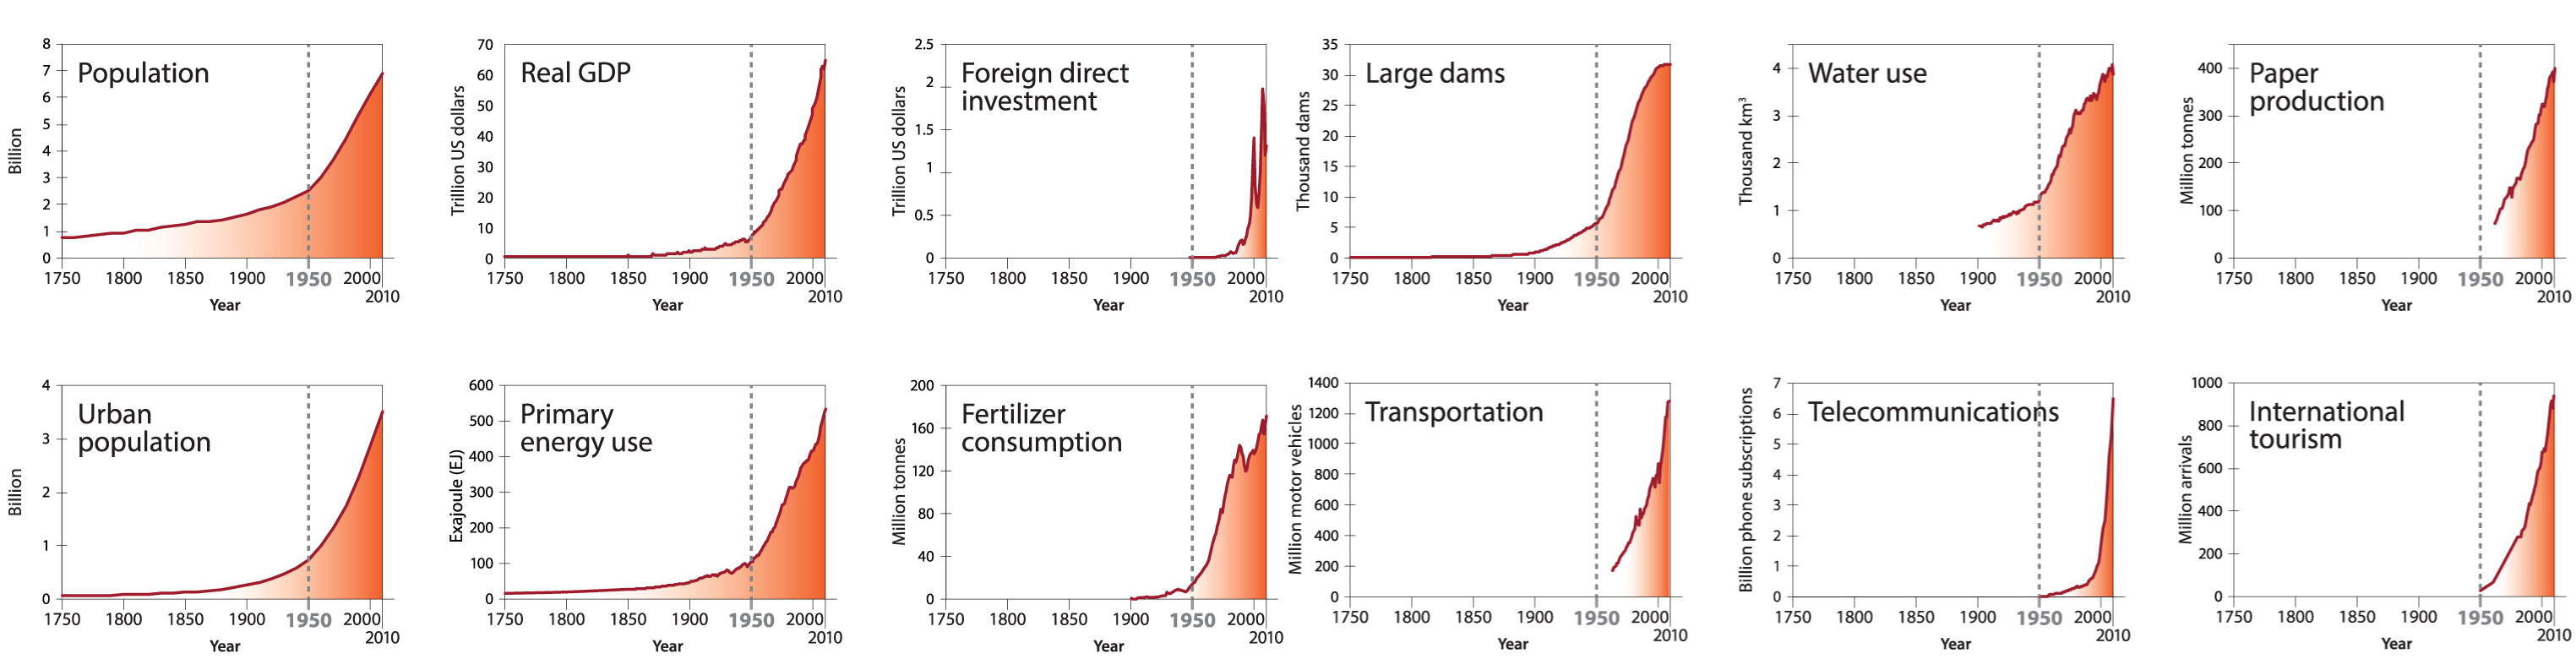
\includegraphics[width=\linewidth]{figures/Anthropocene1V.jpg}
    \caption{Évolution, de 1750 à 2010, de différents indicateurs mondiaux
    du développement socio-économique.}
    \label{fig:anthropocene1}
\end{figure}
 
\begin{figure}[htbp]
    \centering
    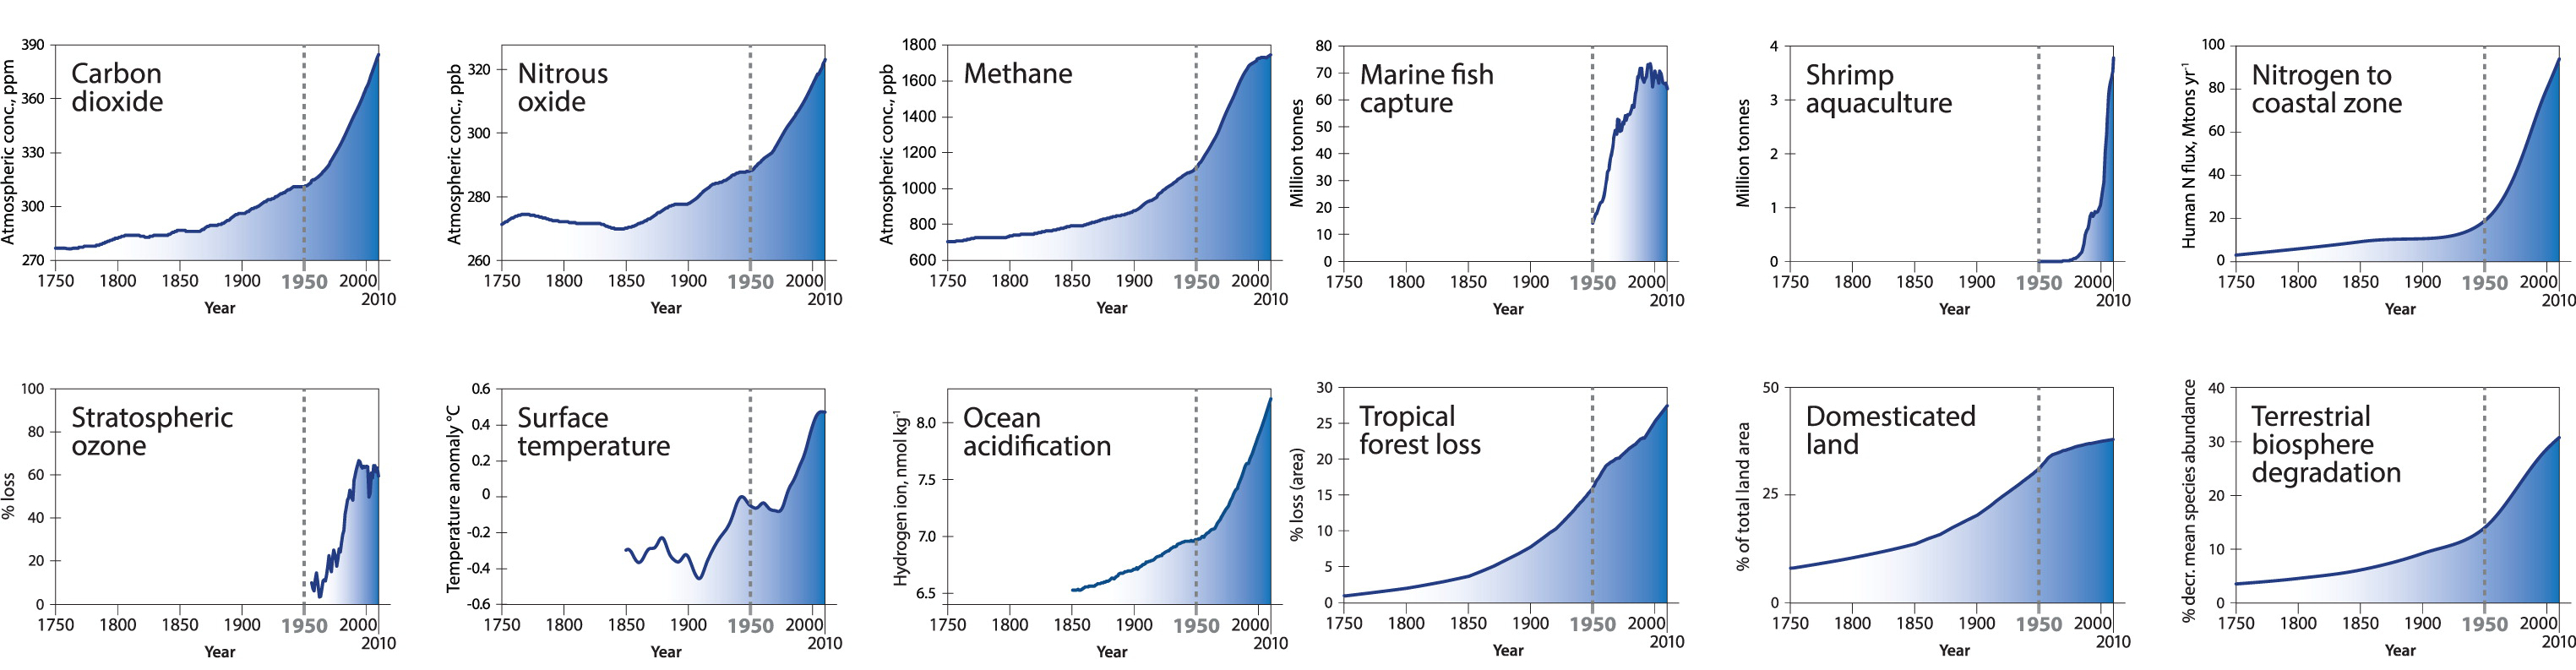
\includegraphics[width=\linewidth]{figures/Anthropocene2V.jpg}
    \caption{Évolution, de 1750 à 2010, de différents indicateurs du
    système terrestre.}
    \label{fig:anthropocene2}
\end{figure}
 
Ces deux séries présentent la même allure : une évolution lente jusqu'au milieu du \textsc{xx}\textsuperscript{e}~siècle, puis une envolée à partir des années 1950. Cette simultanéité, que les auteurs nomment la \emph{Grande Accélération}, met en évidence le lien direct entre la croissance des activités humaines et la dégradation du système terrestre.

\section{Climat}
\subsection*{L'effet de serre}
\label{chap:effet-serre}

\subsubsection*{Mécanisme de l'effet de serre}
Le mécanisme de l'effet de serre peut se décomposer en plusieurs étapes\footfullcite{oce}$^,$\footfullcite{reveilleur-effet-serre}$^,$\footfullcite{ipcc_climate_2021} et est illustré dans la figure~\ref{fig:serre}.
\begin{enumerate}
  \item \textbf{Rayonnement venant du Soleil} : le rayonnement solaire atteint le haut de l'atmosphère.
  \item \textbf{Traversée de l'atmosphère terrestre} : une partie du rayonnement est réfléchie vers l'espace, une autre est transmise vers la surface de la Terre.
  \item \textbf{Arrivée à la surface de la Terre} : une partie du rayonnement est réfléchie vers l'atmosphère, l'autre est absorbée par la surface.
  \item \textbf{Accumulation d'énergie} : la température de la surface terrestre augmente car elle reçoit l'énergie du Soleil.
  \item \textbf{Émission de rayonnement infrarouge} : tous les corps émettent du rayonnement en fonction de leur température\footfullcite{stefan1879}. Les objets chauds rayonnent davantage que les objets froids. La surface de la Terre émet alors un rayonnement infrarouge, qui transporte de la chaleur vers l'atmosphère.
  \item \textbf{Effet de serre} : certains gaz de l'atmosphère absorbent une partie du rayonnement infrarouge, empêchant toute la chaleur de ce rayonnement de s'échapper dans l'espace. Ces gaz chauffent et réémetten de l'infrarouge.
  \item \textbf{Nouvelle absorption par la surface} : la surface de la Terre se réchauffe alors davantage.
\end{enumerate}

\begin{figure}[h]
    \centering
    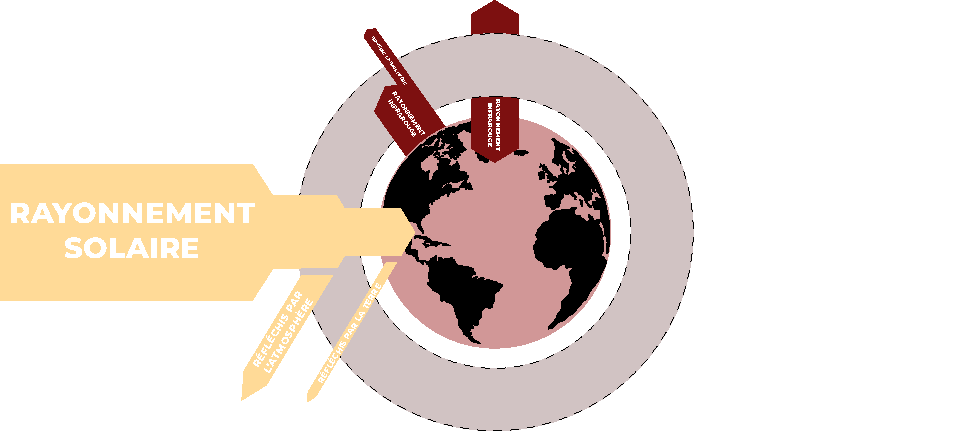
\includegraphics[width=1\linewidth]{figures/serre.pdf}
    \caption{Schéma de principe de l'effet de serre}
    \label{fig:serre}
\end{figure}

La Terre, plus froide que le Soleil, rayonne dans l'infrarouge. Sans effet de serre, la température de la Terre serait à l'équilibre autour de $-18$\,°C. Avec l'effet de serre, la température de la Terre s'équilibre autour de 15\,°C.

Ainsi, l'effet de serre n'est ni « bon » ni « mauvais » : c'est un mécanisme naturel qui maintient la température moyenne de la surface de la Terre. Le principal gaz à effet de serre est la vapeur d'eau. Sa quantité dans l'atmosphère est globalement stable depuis des milliers d'années\footnote{La quantité de vapeur d'eau dans l'air dépend de la température : si l'atmosphère se réchauffe, elle pourra contenir plus de vapeur d'eau avant saturation. Avec le réchauffement climatique, la quantité de vapeur d'eau a tendance à augmenter et donc à amplifier davantage le phénomène de réchauffement.}. La partie suivante montre l'impact de l'être humain sur l'augmentation de la quantité de gaz à effet de serre dans l'atmosphère. C'est cette augmentation de gaz à effet de serre qui augmente le forçage radiatif conduisant la Terre à se réchauffer.

Les gaz à effet de serre sont simplement définis comme les gaz absorbant le rayonnement infrarouge, c'est une propriété intrinsèque à chaque gaz (certains absorbent le rayonnement infrarouge, d'autres non).

\subsubsection*{Limite de l'analogie}
L'effet de serre n'est toutefois pas analogue au fonctionnement d'une serre agricole. Dans une serre agricole fermée, le réchauffement de l'air est issu du rayonnement solaire (qui chauffe le sol) mais surtout de la convection : dans une serre fermée, l'air chaud ne peut pas s'échapper et reste dans la serre.

Ce n'est donc pas la même chose que l'effet de serre, qui est l'émission de rayonnement infrarouge par la Terre, rayonnement qui est absorbé par les gaz à effet de serre contenus dans l'atmosphère. Ce rayonnement absorbé réchauffe l'atmosphère qui, étant plus chaude, rayonne également de l'infrarouge vers l'espace et vers la Terre, conduisant à son réchauffement.

\subsection*{Évolution et contribution anthropique}
La figure~\ref{fig:GES}, issue du GIEC\footfullcite{ipcc_climate_2022}, illustre l'évolution des gaz à effet de serre, cette évolution est due aux différentes activités humaines. Le Secten, réalisé par le Citepa\footfullcite{citepa_secten_2024}, illustre la répartition des GES en France par secteur (figure~\ref{fig:GES2}).
\begin{figure}
    \centering
    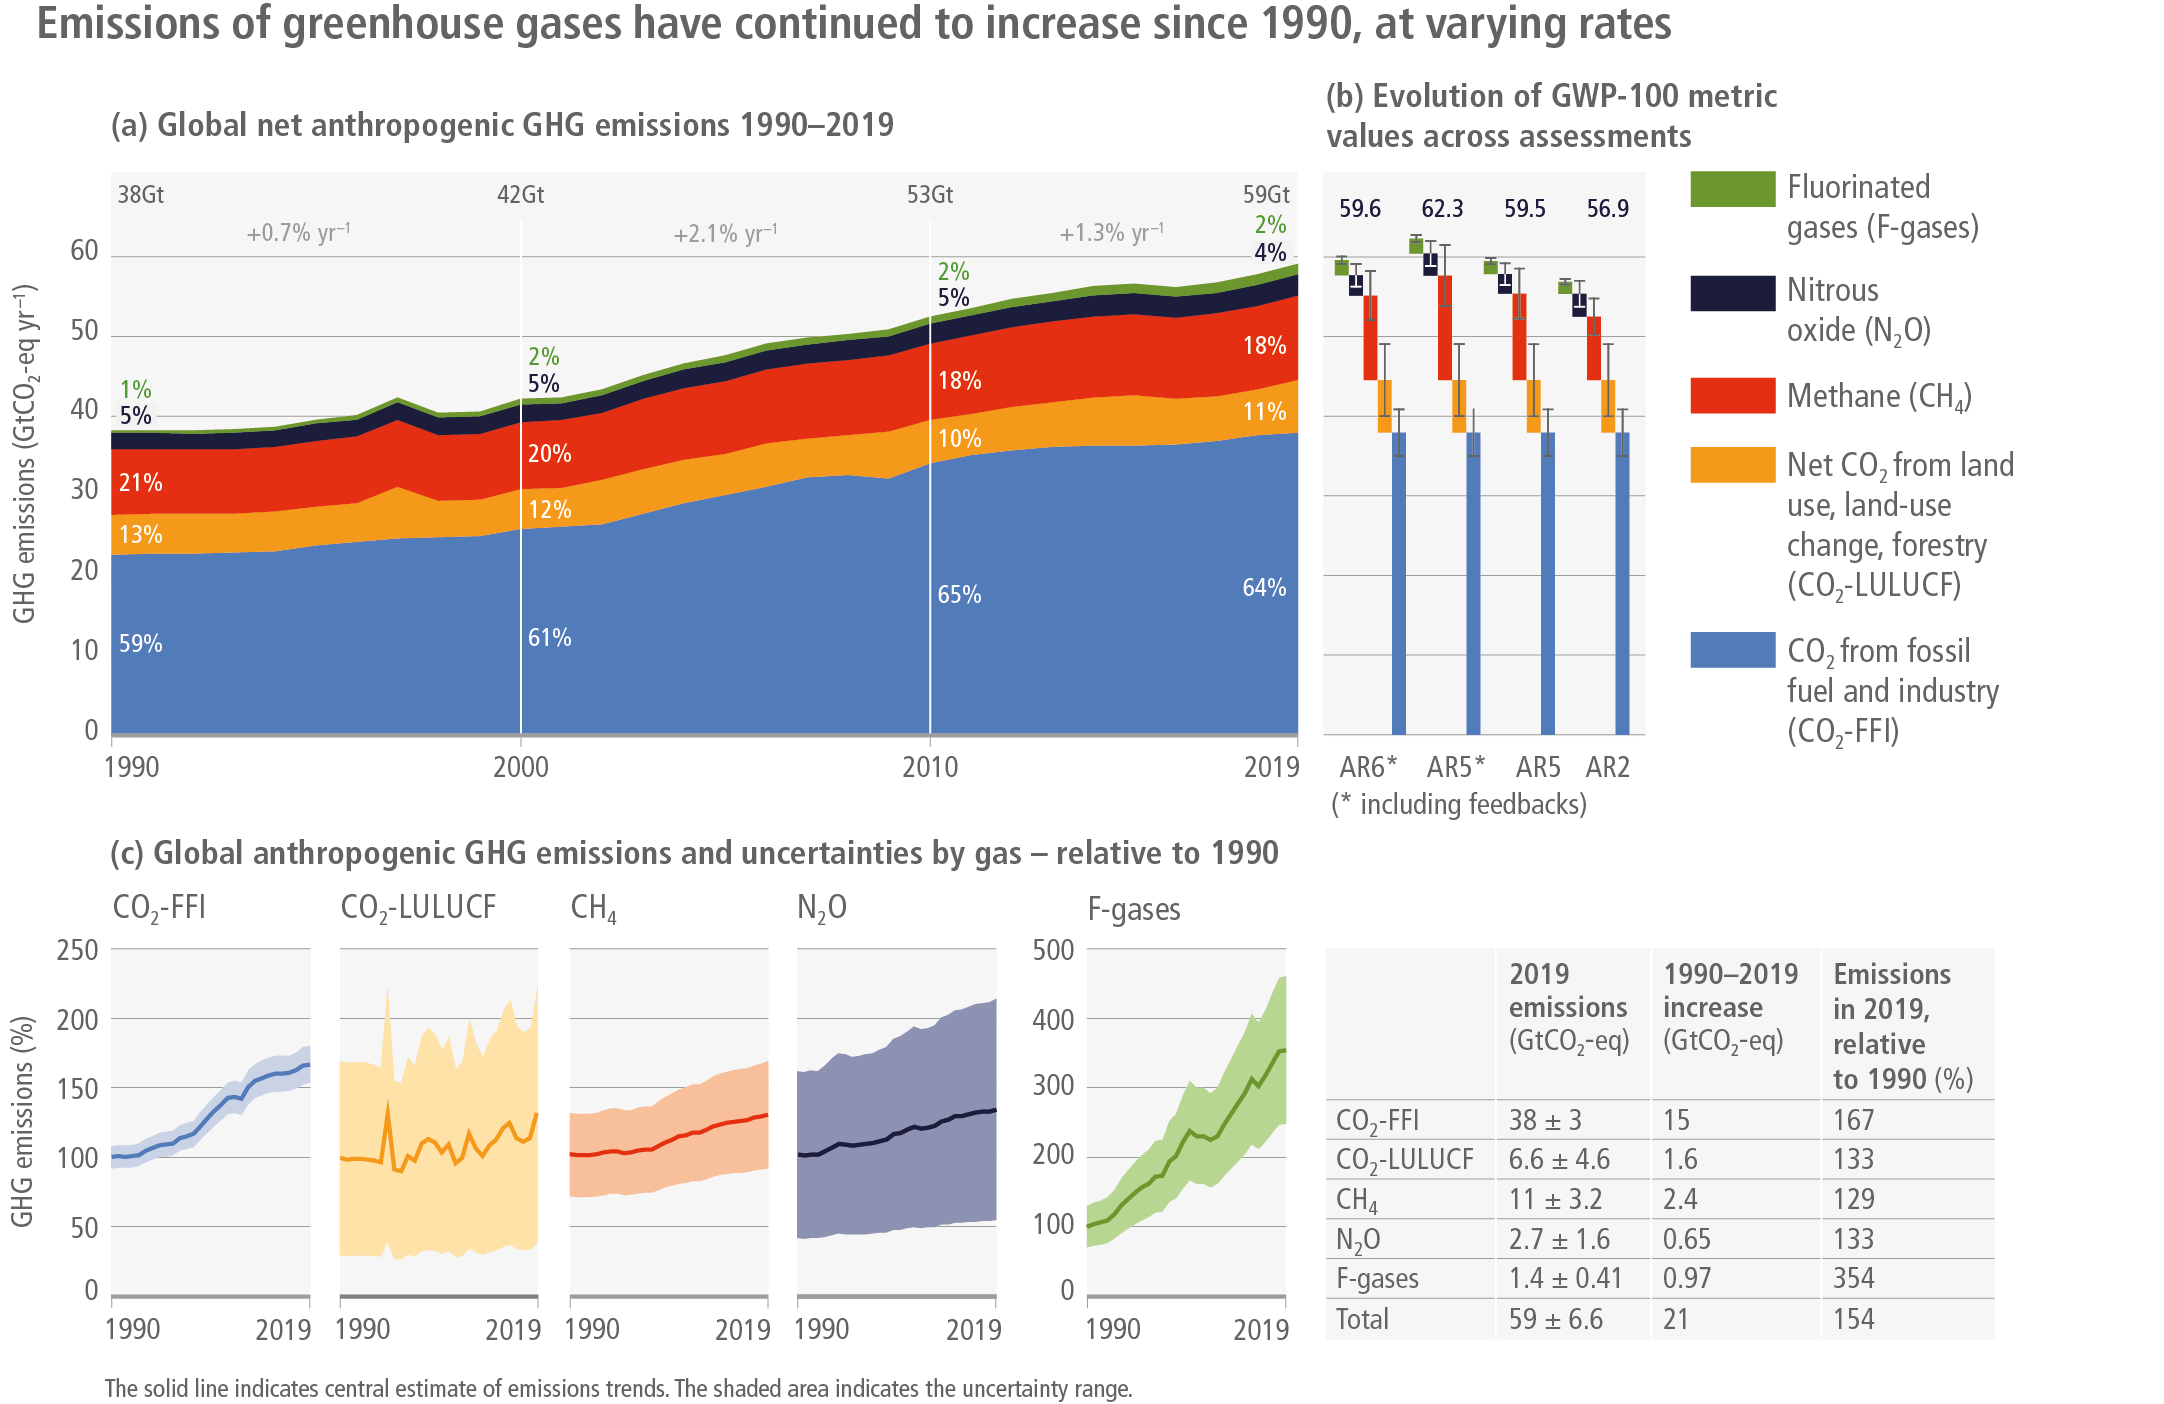
\includegraphics[width=1\linewidth]{figures/GES evolution.png}
    \caption{Évolution anthropique des GES\cite{ipcc_climate_2022}}
    \label{fig:GES}
\end{figure}

\begin{figure}
    \centering
    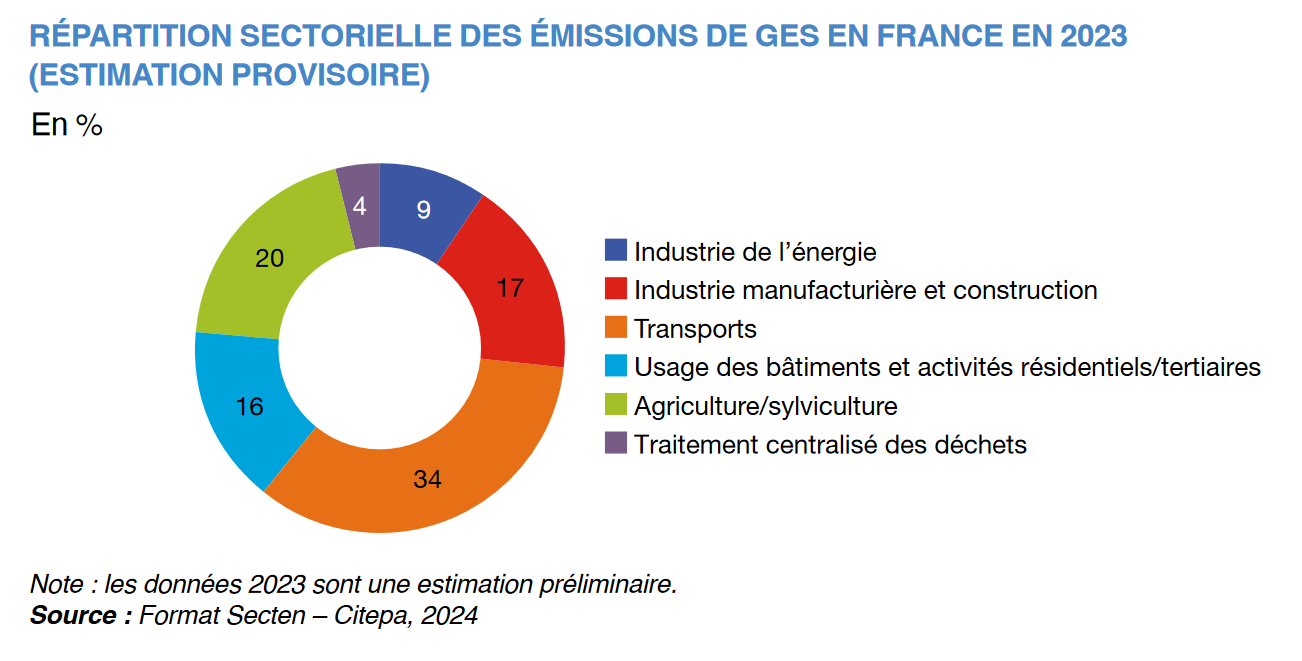
\includegraphics[width=1\linewidth]{figures/ADEME.png}
    \caption{Contribution des GES par secteur en France}
    \label{fig:GES2}
\end{figure}
\subsection*{Atténuation et adaptation face au changement climatique}
On distingue les notions d'atténuation et d’adaptation face au changement climatique (les définitions, différences et rôle en architecture seront détaillés ci-dessous).

\subsubsection*{Atténuation}
Définition (glossaire du GIEC\footfullcite{giec_sr15_glossaire}) : \textit{Intervention humaine visant à réduire les émissions ou à renforcer les puits de gaz à effet de serre.}
\subsubsection*{Adaptation}
Définition (glossaire du GIEC) : \textit{Pour les systèmes humains, démarche d’ajustement au climat actuel ou attendu ainsi qu’à ses conséquences, de manière à en atténuer les effets préjudiciables et à en exploiter les effets bénéfiques. Pour les systèmes naturels, démarche d’ajustement au climat actuel ainsi qu’à ses conséquences. L’intervention humaine peut faciliter l’adaptation au climat attendu et à ses conséquences.}
% TODO : à compléter
\section{Ressources}

Une croissance infinie de la consommation de matières est incompatible avec un monde aux ressources finies. Cette contrainte concerne directement le secteur de la construction, consommateur de granulats, de sable, de métaux et d'énergie fossile\footfullcite{jancovici-blain2021}$^,$\footfullcite{bihouix-perriot2024}.

% FIGURES : Figures/sansfin.jpg et Figures/ressources.jpg

\subsection*{Jour du dépassement}

Le jour du dépassement\footfullcite{gfn-overshootday} compare deux grandeurs\footfullcite{gfn-glossary} :
\begin{itemize}
  \item la \textbf{biocapacité} : la capacité des écosystèmes à fournir des matières biologiques utiles et à assimiler les déchets générés par les êtres humains
  \item l'\textbf{empreinte écologique} : la surface biologiquement productive de terre et d'eau dont un individu, une population humaine ou une activité a besoin pour produire les ressources qu'elle consomme et absorber les déchets qu'elle génère, en utilisant les technologies et les pratiques de gestion des ressources existantes
\end{itemize}

\begin{encadre}{Pour calculer le jour du dépassement}
\begin{itemize}
  \item Individuel : \url{https://www.footprintcalculator.org/fr}
  \item Par pays : \url{https://data.footprintnetwork.org}
\end{itemize}
\end{encadre}

% FIGURE : Figures/Overshoot.png
% FIGURE : Figures/biocapacité.png
%   Biocapacité française

\section{Santé}

La santé concerne à la fois la santé humaine (pollution de l'air, îlots de chaleur, etc.) et celle des écosystèmes (biodiversité, sols, milieux aquatiques). Deux exemples, l'eutrophisation et la formation d'ozone photochimique, sont détaillés avec les indicateurs de l'ACV (partie~3).

% ---------------------------------------------------------------------
\chapter{Impact du secteur du bâtiment}

% FIGURE : Figures/fallingwater.jpg
%   Maison sur la Cascade, Frank Lloyd Wright, 1939. Crédit Britannica
% FIGURE : Figures/fallingwater_R
%   Maison sur la Cascade, chantier de rénovation (2025 ?). Crédit Jason Nark / The Philadelphia Inquirer

\section{Impact du secteur du bâtiment dans le monde}

En 2019, le secteur du bâtiment représente 21\,\% des émissions mondiales de gaz à effet de serre (GES)\footfullcite{ipcc_climate_2022}. Ces émissions se décomposent en :
\begin{itemize}
  \item 57\,\% liées à la production d'électricité et de chaleur (exploitation)
  \item 24\,\% liées à la construction
  \item 18\,\% liées aux matériaux, essentiellement le béton et l'acier
\end{itemize}

Entre 1990 et 2019, les émissions de GES du bâtiment ont augmenté de 50\,\% et sa consommation électrique de 138\,\%.

\section{Impact du secteur du bâtiment en France}

En 2017, le secteur du bâtiment représente 23\,\% des émissions de GES en France\footfullcite{ademe-batiments}. Pour les bâtiments neufs, 70\,\% de ces émissions sont liées à la phase de construction (chantier et matériaux).

Le secteur du bâtiment représente également 45\,\% de la consommation énergétique nationale.

% ---------------------------------------------------------------------
\chapter{Cadre réglementaire, la RE 2020}

\section{Présentation}

La France s'est dotée d'une réglementation environnementale en 2022, qui prend progressivement la suite de la RT 2012 : la RE 2020. Nous passons d'une Réglementation Thermique (RT) à une Réglementation Environnementale (RE).

Elle poursuit des objectifs d'amélioration de la performance énergétique des bâtiments neufs, de réduction de leur impact sur le climat (prise en compte des émissions de gaz à effet de serre sur l'ensemble du cycle de vie des bâtiments) et de leur adaptation aux conditions climatiques futures (renforcement du confort d'été)\footfullcite{guide-re2020}.

\subsection*{Catégories et indicateurs}

La RE 2020 s'articule autour de trois catégories (carbone, énergie, confort d'été) et de six indicateurs (tableau~\ref{tab:re2020-indicateurs}).

\begin{table}[htbp]
\centering
\caption{Les six indicateurs de la RE 2020}

\small
\renewcommand{\arraystretch}{1.25}
\begin{tabular}{p{1.6cm}p{2.6cm}p{3.8cm}p{6cm}}
\textbf{Catégorie} & \textbf{Indicateur} & \textbf{Définition} & \textbf{Description} \\
\hline
Carbone & $I_c$ construction (kgeqCO$_2$/m$^2$) & Impact sur le changement climatique associé aux « composants » et au « chantier » & Utilisation de la méthode d'Analyse de Cycle de Vie pour l'évaluation des émissions de gaz à effet de serre. \\
\cline{2-4}
 & $I_c$ énergie (kgeqCO$_2$/m$^2$) & Impact sur le changement climatique associé aux consommations d'énergie primaire & Utilisation de la méthode d'Analyse de Cycle de Vie pour l'évaluation des émissions de gaz à effet de serre concernant l'énergie consommée pendant le fonctionnement du bâtiment. \\
\hline
Énergie & $C_{ep}$ (kWhep/(m$^2$.an)) & Consommation d'énergie primaire totale & Évaluation de la consommation d'énergie primaire durant la vie du bâtiment. \\
\cline{2-4}
 & $C_{ep,nr}$ (kWhep/(m$^2$.an)) & Consommation d'énergie primaire non renouvelable & Évaluation de la consommation d'énergie non renouvelable durant la vie du bâtiment. \\
\cline{2-4}
 & $B_{bio}$ (points) & Besoins bioclimatiques & Évaluation des besoins de chaud, de froid et d'éclairage. \\
\hline
Confort d'été & DH (°C.h) & Degrés-heures d'inconfort : niveau d'inconfort perçu par les occupants sur l'ensemble de la saison chaude & Évaluation des écarts entre la température du bâtiment et la température de confort. \\
\hline
\end{tabular}
\label{tab:re2020-indicateurs}
\end{table}


\subsection*{Progressivité}

La RE 2020 est entrée en vigueur le 1\textsuperscript{er} janvier 2022 pour les maisons individuelles et les logements collectifs, puis elle a progressivement intégré différents usages. À partir du 1\textsuperscript{er} mai 2026, quasiment tous les programmes de constructions neuves sont concernés. L'application de la RE 2020 aux projets de rénovation n'est actuellement ni prévue ni annoncée, mais cela peut bien entendu évoluer (à suivre).
Pour chaque indicateur, la RE 2020 fixe un seuil à ne pas dépasser. Les seuils carbone et énergie sont renforcés en plusieurs phases : 2025, 2028 puis 2031.

\section{Les indicateurs carbone}

L'ACV est imposée dans le cadre de la RE 2020 pour la catégorie carbone, via les deux indicateurs Ic construction et Ic énergie.

\subsection*{Ic construction}
L'Ic construction (kgeqCO$_2$/m$^2$) représente l'impact de la construction sur le changement climatique. Il prend en compte les matériaux, les équipements ainsi que leur mise en œuvre sur le chantier : un bilan carbone sur les matériaux, les équipements et le chantier est à effectuer en prenant en compte tout le cycle de vie du bâtiment (du transport des matériaux lors de leur fabrication jusqu'à la démolition de l'ouvrage). Les seuils moyens sont évolutifs et donnés par typologie de programme dans le tableau~\ref{tab:ic-construction}.

\begin{table}[h]
\centering
\caption{Seuils Ic\,construction,maxmoyen (kgCO$_2$e/m$^2$)}
\label{tab:ic-construction}
\begin{tabular}{lcccc}
\hline
Usage & 2022 & 2025 & 2028 & 2031 \\
\hline
Logement & 740 & 650 & 580 & 490 \\
Bureau & 980 & 810 & 710 & 600 \\
Enseignement & 900 & 770 & 680 & 590 \\
\hline
\end{tabular}
\end{table}

\subsection*{Ic énergie}
L'Ic énergie (kgeqCO$_2$/m$^2$) représente l'impact de l'énergie sur le changement climatique (il prend en compte la consommation d'énergie et d'eau). Un bilan carbone est à effectuer en prenant en compte l'impact carbone de la production d'énergie et d'eau utilisées dans le bâtiment durant toute sa durée de vie. Les seuils moyens sont donnés dans le tableau~\ref{tab:ic-energie}.

\begin{table}[h]
\centering
\caption{Seuils Ic\,énergie,maxmoyen (kgCO$_2$e/m$^2$)}
\label{tab:ic-energie}
\begin{tabular}{lccc}
\hline
Usage & 2022 & 2025 & 2028 \\
\hline
Logement & 560 & 320 & 260 \\
Bureau & 280 & 200 & -- \\
Enseignement primaire et secondaire & 240 & 200 & 140 \\
\hline
\end{tabular}
\end{table}

Le calcul de ces deux indicateurs repose sur une ACV dynamique, présentée dans la partie~4.

\section{Énergie}

\subsection*{Énergie primaire} L'énergie primaire est une forme d'énergie disponible dans la nature avant toute transformation\footfullcite{sdes-energie}\footnote{\texttt{https://www.statistiques.developpement-durable.gouv.fr/}}. L'évolution de la consommation d’énergie primaire de la France est présentée sur la figure~\ref{fig:primaire} et sa répartition est détaillée ci-dessous :
\begin{itemize}
  \item 43\,\% de nucléaire
  \item 26\,\% de pétrole
  \item 12\,\% de gaz naturel
  \item 16\,\% d'énergies renouvelables et déchets (dont 1\,\% de déchets non renouvelables)
  \item 2\,\% de charbon
\end{itemize}


\begin{figure}
    \centering
    \includesvg[width=0.5\linewidth]{figures/primaire.svg}
    \caption{Évolution de la consommation d’énergie primaire française}
    \label{fig:primaire}
\end{figure}

\subsection*{Consommation d'énergie primaire}
La consommation d'énergie primaire $C_{ep}$ (kWhep/(m$^2$.an)) est estimée pour le bâtiment et doit être inférieure à certains seuils, voir tableau~\ref{tab:cep-seuils}.

\subsection*{Consommation d'énergie primaire non renouvelable}
De même, la consommation d'énergie primaire non renouvelable $C_{ep,nr}$ (kWhep/(m$^2$.an)) doit être inférieure à un certain seuil. La RE 2020 distingue le $C_{ep}$ du $C_{ep,nr}$ pour favoriser l'utilisation d'énergie renouvelable, et assurer des bâtiments plus sobres en consommation d'énergie (ce n'est pas parce que l'énergie est renouvelable que l'on veut la gaspiller).

\begin{table}[htbp]
\centering
\caption{Seuils de consommation d'énergie primaire (kWhep/(m$^2$.an))}
\label{tab:cep-seuils}
\begin{tabular}{l|c|c}

\textbf{Usage} & \textbf{$C_{ep,\mathrm{maxmoyen}}$} & \textbf{$C_{ep,nr,\mathrm{maxmoyen}}$} \\
\hline
Logement collectif & 85 & 70 \\
Bureau & 85 & 75 \\
Enseignement primaire & 72 & 65 \\

\end{tabular}
\end{table}

\subsection*{Besoin bioclimatique}
Le calcul du $B_{bio}$ RE 2020 comprend les besoins en chauffage, en refroidissement et en éclairage du bâtiment.
Le $B_{bio}$ s'intéresse au bâti sans ses équipements.

Le $B_{bio}$ s'intéresse à :
\begin{itemize}
  \item l'orientation
  \item l'isolation
  \item la compacité
  \item les surfaces vitrées
  \item la protection solaire
  \item l'inertie
  \item la conception globale de l'enveloppe
\end{itemize}

Le $B_{bio}$ est une note en points, calculée pendant la conception du bâtiment.

\section{Confort d'été}
\subsection*{Degrés-heures d'inconfort}

Chaque heure, on compte l'écart entre la température du bâtiment et la température limite de confort.
Le calcul des degrés-heures d'inconfort (DH) suit les étapes suivantes, et est illustré figure~\ref{fig:dh} :

\begin{enumerate}
  \item La température extérieure est estimée à partir de fichiers météo prenant en compte des scénarios caniculaires.
  \item Un calcul de la température du bâtiment est effectué (simulation avec un logiciel spécialisé).
  \item On regarde pour chaque heure si la température du bâtiment dépasse la température de confort, si oui on compte de combien de degrés elle dépasse la température de confort.
\end{enumerate}

\begin{figure}
    \centering
    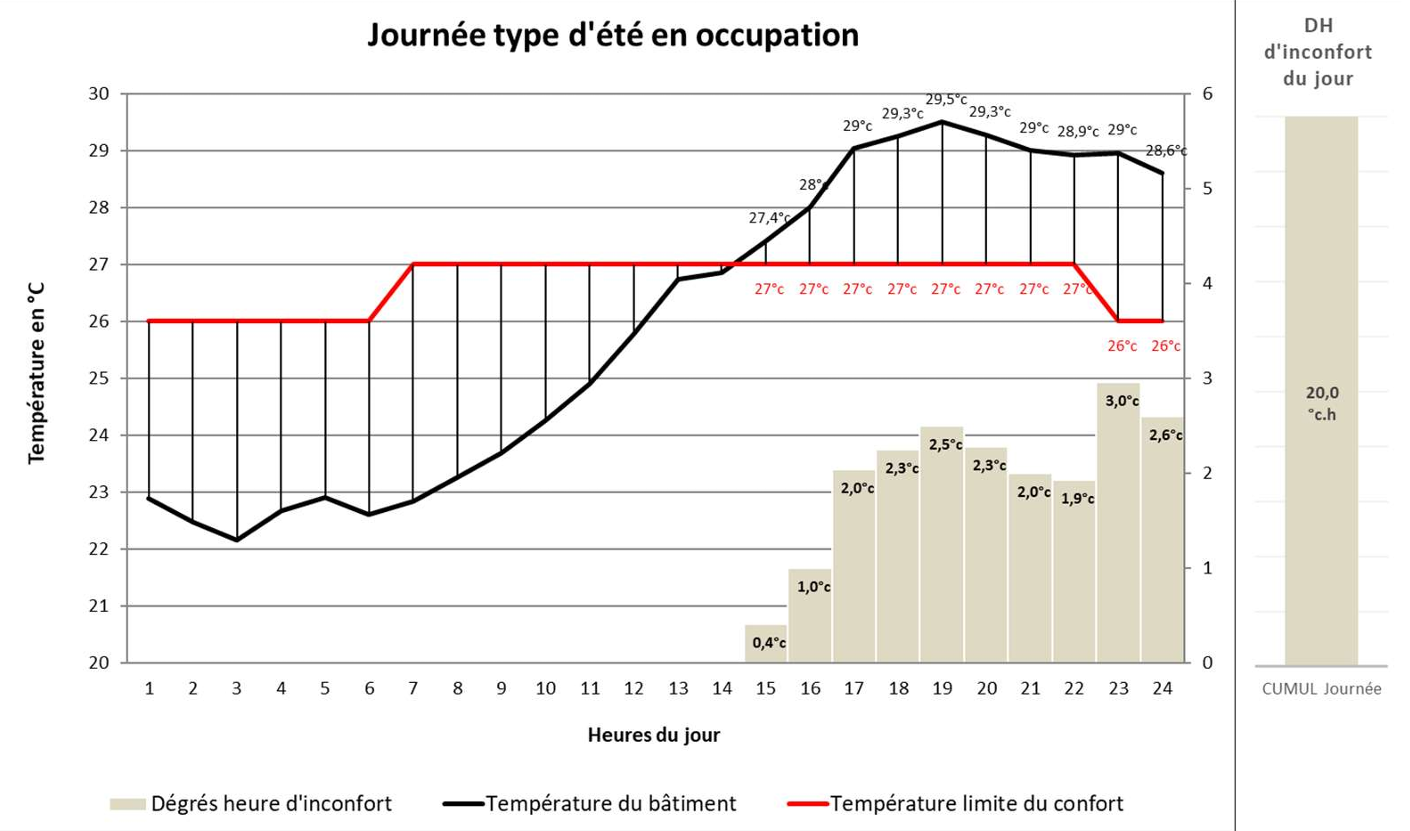
\includegraphics[width=0.5\linewidth]{figures/DH.png}
    \caption{Degrés-heures issus du Guide de la RE 2020 \footfullcite{guide-re2020}}
    \label{fig:dh}
\end{figure}

\section{Conclusion sur la RE 2020}
La RE 2020 est la réglementation environnementale en vigueur pour les projets neufs, elle se compose de 6 indicateurs qui doivent respecter les seuils (évolutifs). Ces 6 indicateurs sont regroupés en trois catégories : carbone, énergie et confort d'été, comme illustré sur le schéma~\ref{fig:20}.

\begin{figure}
    \centering
    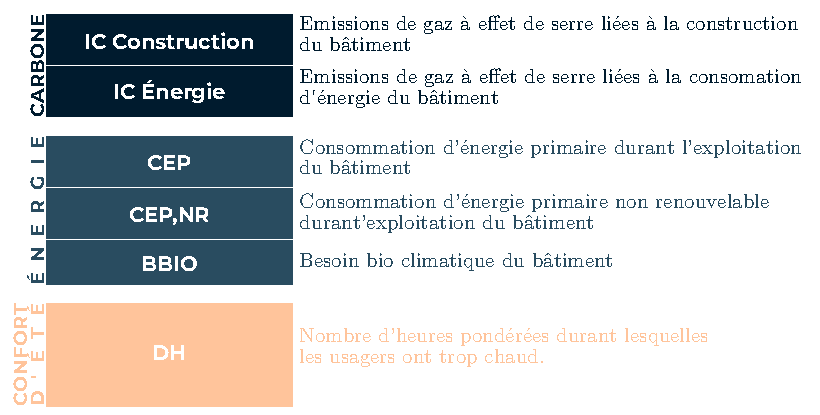
\includegraphics[width=1\linewidth]{figures/re.pdf}
    \caption{Synthèse des indicateurs de la RE 2020}
    \label{fig:20}
\end{figure}

\chapter{Conclusion sur le contexte}

% =====================================================================
%  Partie 2 — Méthode de l'ACV
%  Les figures des diapositives sont signalées en commentaire « FIGURE ».
% =====================================================================
\part{Méthode générique de l'ACV}

% ---------------------------------------------------------------------
\chapter{Historique et présentation}
La méthode de l'analyse de cycle de vie n'est pas propre à l'architecture, au contraire. Cette section détaille tout d'abord la méthode générique de l'ACV, pour ensuite faire les parallèles et applications à l'architecture.
\section{Historique}

\begin{itemize}
  \item \textbf{1969} : Coca-Cola réalise une étude comparative de différents emballages, un des premiers exemples d'analyse multicritère\footfullcite{feraille_analyse_2022}.
  \item \textbf{1972} : le rapport Meadows, \textit{The Limits to Growth}, met en exergue les dangers, pour l'environnement et donc l'humanité, de la croissance économique et démographique que connaît le monde.
  \item \textbf{1970-1987} : différents chocs pétroliers favorisent le développement des bilans énergétiques et des premières approches d'évaluation sur le cycle de vie (\textit{Bilan produit} en Europe, \textit{REPA} aux États-Unis).
  \item \textbf{1997} : la méthode d'ACV est normalisée par l'ISO.
  \item \textbf{2000-2010} : l'ACV se démocratise et commence à s'intégrer au secteur du bâtiment. Les produits de construction sont évalués à travers les FDES.
  \item \textbf{2020} : la RE 2020 introduit l'ACV dans la réglementation française de la construction neuve.
\end{itemize}

\section{Présentation}

L'analyse du cycle de vie (ACV) est une méthode d'évaluation qui permet de réaliser un bilan environnemental multicritère d'un système (produit, service ou procédé) sur l'ensemble de son cycle de vie : extraction des matières premières, fabrication, transport, distribution, utilisation, fin de vie, valorisation.

Elle repose sur trois approches : multi-étapes, multicritère et comparative.

\subsection*{Approche multi-étapes}
L'ACV prend en compte l'ensemble du cycle de vie, dans le but d'éviter les transferts de pollution d'une étape à l'autre. On évalue les impacts d'un produit du berceau à la tombe (\textit{cradle to grave}).


\subsection*{Approche multicritère}
L'ACV prend en compte plusieurs impacts environnementaux, pour éviter de remplacer un problème par un autre (transfert d'impact). On cherche à couvrir « tous » les problèmes environnementaux : atteintes aux ressources naturelles, à la santé et à la biodiversité.


\subsection*{Approche comparative}

L'ACV permet de comparer plusieurs produits répondant à la même fonction. Le calcul des émissions, extractions et impacts est rapporté à une fonction définie appelée \textbf{unité fonctionnelle}.

La norme ISO 14044 définit l'unité fonctionnelle comme la « performance quantifiée d'un système de produits, destinée à être utilisée comme unité de référence dans une ACV ». En ACV, on ne compare pas des objets : on compare la même fonction rendue par des objets ou systèmes différents. L'unité fonctionnelle est la traduction mesurable de cette fonction.

% ---------------------------------------------------------------------
\chapter{Fonctionnement général de l'ACV}
Une ACV générique (appliquée à un produit ou un service) nécessite les 4 étapes suivantes :
\begin{enumerate}
  \item \textbf{Définition des objectifs et du champ de l'étude} : frontières du système, unité fonctionnelle, hypothèses.
  \item \textbf{Analyse de l'inventaire} : inventorier les émissions et extractions, préciser certains choix de modélisation.
  \item \textbf{Caractérisation des impacts} : choix d'une méthode d'impacts, normalisation et pondération éventuelles.
  \item \textbf{Interprétation des résultats} : analyses de sensibilité, d'incertitude, modifications du modèle.
\end{enumerate}


\section{Indicateurs}

\subsection*{Les indicateurs des FDES}

Les Fiches de Déclaration Environnementale et Sanitaire (FDES, voir partie~4) contiennent 36 indicateurs, que l'on peut regrouper en trois familles :

\paragraph{Climat}
\begin{itemize}
  \item Changement climatique (kg éq. CO$_2$) : fossile, biogénique, usage des sols.
\end{itemize}

\paragraph{Ressources et circularité}
\begin{itemize}
  \item Épuisement des ressources : minéraux et métaux (kg éq. Sb), fossiles (MJ).
  \item Énergie primaire (MJ) : renouvelable et non renouvelable, chacune hors matière, matière et totale.
  \item Matières secondaires (kg).
  \item Combustibles secondaires (MJ) : renouvelables et non renouvelables.
  \item Eau : utilisation nette d'eau douce (m$^3$), privation (m$^3$ éq. de privation).
  \item Déchets éliminés (kg) : dangereux, non dangereux, radioactifs.
  \item Flux de valorisation (kg) : composants pour réutilisation, matériaux pour recyclage, matériaux pour récupération d'énergie.
  \item Énergie exportée (MJ).
\end{itemize}

\paragraph{Santé et écosystèmes}
\begin{itemize}
  \item Santé humaine : particules fines (incidence de maladies), rayonnements ionisants (kBq éq. U-235), toxicité humaine cancérogène et non cancérogène (CTUh), appauvrissement de l'ozone (kg éq. CFC-11), formation d'ozone photochimique (kg éq. COV non méthaniques).
  \item Qualité des écosystèmes : acidification (mol éq. H$^+$), eutrophisation des eaux douces (kg éq. P), marine (kg éq. N) et terrestre (mol éq. N), écotoxicité des eaux douces (CTUe), utilisation et qualité des sols (points).
\end{itemize}

\subsection*{Comparer des impacts différents}

\begin{displayquote}
« Comment comparer toxicité humaine et effet de serre ? En d'autres mots, comparer des pommes et des poires ? Certains diront que ce ne sont pas des pommes et des poires, mais des pommes et des éléphants tellement ces impacts diffèrent. »\footfullcite{saade_analyse_nodate}
\end{displayquote}

Une ACV produit des dizaines d’indicateurs exprimés dans des unités différentes : on ne peut pas additionner des kg éq. CO$_2$, des m$^3$ d’eau et des kg de déchets. Pour comparer deux variantes de projet sur l’ensemble de ces critères, des méthodes d’agrégation ont été développées, comme ReCiPe ou IMPACT World+. Elles regroupent les indicateurs en quelques grandes catégories de dommages (santé humaine, qualité des écosystèmes, ressources), puis peuvent les pondérer pour obtenir un score unique. Cette pondération repose toutefois sur des choix de valeurs (quel poids donner à l’eau par rapport au climat ?), ce qui explique qu’elle reste un sujet de recherche actif et débattu.

\section{Limites}

\subsection*{Allocation}

Le problème de multifonctionnalité, parfois appelé allocation, provient du fait qu'un même procédé peut générer plusieurs produits, et donc répondre à plusieurs fonctions. Comment allouer l'inventaire (puis les impacts) du procédé à ces différents produits ? La méthode de partitionnement des procédés, parfois appelée méthode de l'allocation, est l'une des méthodes pour résoudre ce problème, parmi d'autres (expansion du système, méthode de substitution, etc.).

L'exemple du haut fourneau, qui produit à la fois de l'acier et du laitier, montre que le choix de la clé de répartition modifie le résultat, selon que l'on répartit les émissions selon la masse ou selon le prix des produits.

\subsection*{Données}

L'inventaire d'un bâtiment nécessite des données sur chacun de ses produits et procédés de construction. Ces données sont présentées dans la partie~4. La bonne intégrité de ces données est donc nécessaire à une ACV rigoureuse et pertinente.

\subsection*{Optimisation multicritère}

Il y a plusieurs indicateurs environnementaux et plusieurs méthodes d'agrégation. Chaque méthode d'agrégation fournit des scores différents : il n'existe pas un unique score environnemental.

\subsection*{Optimisation et architecture}

Une évaluation environnementale ne suffit pas à elle seule à arbitrer toutes les valeurs engagées dans un projet d'architecture.

\begin{displayquote}
« Une condition préalable à toute comparaison dans le cadre d'une ACV est que l'“unité fonctionnelle” et que la qualité du ou des produits alternatifs soient identiques (on ne peut comparer des pommes et des oranges). Toutefois, en matière de conception et d'architecture, cette condition semble constituer un défaut fondamental dans l'application de l'ACV : le concepteur ou l'architecte vise une qualité supérieure (au sens large du terme, incluant des aspects immatériels tels que l'esthétique et l'image) : par conséquent, la nouvelle conception ne présente jamais la même qualité que l'ancienne solution. »\footfullcite{vogtlander_practical_2010}
\end{displayquote}

L'unité fonctionnelle ne mesure pas la qualité architecturale et ne permet pas de comparer des projets à « qualité » égale. L'ACV compare des projets à fonction égale. Fonction et qualité architecturale sont deux notions différentes.

\chapter{Conclusion générique sur l'ACV}

% =====================================================================
%  Partie 3 — ACV et architecture
%  Les figures des diapositives sont signalées en commentaire « FIGURE ».
% =====================================================================
\part{ACV et architecture}

% ---------------------------------------------------------------------
\chapter{Méthode d'ACV de bâtiment}
\label{chap:methode-batiment}
\section{Indicateurs}

Dans le domaine du bâtiment, la norme EN 15804+A2 définit 13 indicateurs principaux :
\begin{itemize}
  \item changement climatique total, fossile, biogénique et lié à l'usage des terres (kg CO$_2$ éq.)
  \item appauvrissement de la couche d'ozone (kg CFC-11 éq.)
  \item acidification (mol H$^+$ éq.)
  \item eutrophisation des eaux douces (kg P éq.), marine (kg N éq.) et terrestre (mol N éq.)
  \item formation d'ozone photochimique (kg NMVOC éq.)
  \item épuisement des ressources minérales et métalliques (kg Sb éq.)
  \item épuisement des ressources fossiles (MJ)
  \item utilisation de l'eau (m$^3$ éq. de privation)
\end{itemize}

Aucune méthode d’agrégation n’est imposée réglementairement : actuellement, la RE 2020 n’exige qu’une ACV portant sur le seul changement climatique.

Notons qu'une solution qui réduit le carbone peut en dégrader d’autres : c’est ce qu’on appelle un transfert d’impact (par exemple, un isolant bas carbone mais plus consommateur). Pour s’en prémunir, l’architecte peut regarder au-delà du carbone, soit en choisissant lui-même quelques indicateurs pertinents pour son projet, soit en s’appuyant sur une méthode d’agrégation, en gardant à l’esprit ses hypothèses de pondération.

Pour aller plus loin : la méthode \emph{Environmental Footprint}\footfullcite{andreasibassi2023ef31}, développée par le Centre commun de recherche (JRC) de la Commission européenne, présente un intérêt particulier pour l'architecte : ses indicateurs sont ceux des FDES (voir partie suivante). Il est donc possible, à partir des valeurs disponibles sur la base INIES, d'appliquer ses facteurs de normalisation et de pondération pour obtenir un score environnemental unique, et ainsi comparer des variantes de projet au-delà du seul critère carbone. Le lecteur curieux pourra consulter le rapport de référence du JRC\footnote{\url{https://publications.jrc.ec.europa.eu/repository/handle/JRC130796}}. Il gardera à l'esprit que toute pondération repose sur des choix de valeurs : un score unique aide à décider, mais ne remplace pas l'examen des indicateurs détaillés.

\section{Modules}

Le cycle de vie d'un bâtiment est découpé en 4 modules (A, B, C et D), illustrés figure~\ref{fig:module}.
\begin{figure}[h]
    \centering
    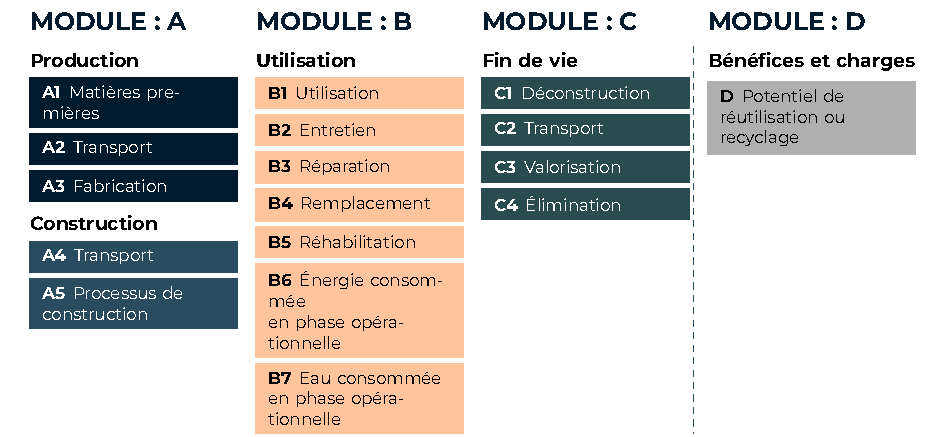
\includegraphics[width=1\linewidth]{figures/Modules.pdf}
    \caption{Modules de l'ACV de bâtiment}
    \label{fig:module}
\end{figure}

Les modules A couvrent l’amont et la construction. Les modules A1 à A3 correspondent à la production (ils incluent l’extraction des matières premières, le transport vers l’usine et la fabrication des produits). Les modules A4 et A5 correspondent à la construction du bâtiment (transport jusqu’au chantier et pose). Les modules B portent sur l’exploitation (usage, maintenance, réparation et remplacement). Enfin, les modules C traitent de la fin de vie (déconstruction, transport des déchets et traitement).

Le module D se situe au-delà de la frontière du système : il dépasse le cycle de vie du bâtiment et comptabilise les bénéfices et charges liés à la valorisation après la fin de vie. Cela concerne le réemploi, le recyclage et la récupération d’énergie. Par exemple, un matériau recyclable peut générer un crédit environnemental.

On distingue deux périmètres, selon que l'on souhaite étudier l'ensemble du cycle de vie du bâtiment ou uniquement sa construction. Ce choix n'est pas neutre : les impacts de la construction dépendent en grande partie des choix de conception de l'architecte (système constructif, matériaux, quantités), alors que les impacts liés à l'exploitation du bâtiment dépendent aussi des équipements et des consommations d'énergie, qui relèvent de l'ensemble de la maîtrise d'œuvre, et notamment des bureaux d'études :
\begin{itemize}
  \item \textbf{du berceau à la porte} (\textit{cradle to gate}) : en bâtiment, du berceau à la livraison, les modules A1 à A5
  \item \textbf{du berceau à la tombe} (\textit{cradle to grave}) : tout le cycle de vie, des modules A1 à C4, voire D
\end{itemize}


\section{FDES}

Les Fiches de Déclaration Environnementale et Sanitaire (FDES) sont encadrées par la norme NF EN 15804+A1 et le complément national NF EN 15804 CN. Elles sont issues d'un résultat d'analyse de cycle de vie sur les produits et les procédés de construction. Elles contiennent :
\begin{itemize}
  \item des informations générales (dates, constructeurs, scénarios, etc.)
  \item l'unité fonctionnelle et la durée de vie de référence
  \item un tableau d'indicateurs environnementaux
  \item des données de contribution à la santé et au confort
\end{itemize}

\textbf{Les FDES permettent aux architectes de réaliser l'ACV d'un projet sans avoir à faire l'analyse de l'inventaire.}

\subsection*{Types de FDES}

Il existe 5 types de FDES\footfullcite{inies} :
\begin{itemize}
  \item \textbf{individuelles} : un déclarant pour un produit
  \item \textbf{individuelles de gamme} : un déclarant pour une gamme de produits
  \item \textbf{collectives} : un groupe de déclarants pour un produit ou une gamme de produits
  \item \textbf{paramétrables} : on peut paramétrer les déclarations de différents produits
  \item \textbf{données environnementales par défaut} : elles sont mises à disposition par le ministère en charge de la construction en l'absence de données spécifiques
\end{itemize}

\subsection*{Configurateurs de FDES}

Les FDES paramétrables se génèrent à l'aide de configurateurs présentés dans le tableau~\ref{tab:configurateurs}.

\begin{table}[h]
\centering
\small
\caption{Configurateurs de FDES paramétrables}
\label{tab:configurateurs}
\begin{tabular}{lll}
\textbf{Configurateur} & \textbf{Produits} & \textbf{Adresse} \\

\noalign{\vskip 4pt}
\multicolumn{3}{c}{\textit{Gros œuvre et structure}} \\
\cline{1-3}
\noalign{\vskip 2pt}
Betie & béton prêt à l'emploi & \url{https://www.snbpe.org/betie-4-0/} \\
Environnement IB & béton préfabriqué & \url{http://www.environnement-ib.com/} \\
PHARE & bétons Hoffmann & \url{https://calculateurco2.ciments-hoffmann.fr/} \\
DE-Bois & construction bois & \url{https://www.de-bois.fr/} \\
DE-Bois de France & bois français & \url{https://www.de-boisdefrance.fr/} \\
SAVE & construction acier & \url{https://www.save-construction.com/} \\
DIMACV & pierre naturelle & \url{https://dimacv.ctmnc.fr/} \\
\noalign{\vskip 10pt}
\multicolumn{3}{c}{\textit{Enveloppe et aménagement}} \\
\cline{1-3}
\noalign{\vskip 2pt}
AGC Glass & vitrages & \url{https://www.agc-yourglass.com/fr-FR/} \\
Config'Alu & aluminium, garde-corps & \url{https://configalu.batir-en-alu.fr/} \\
DE-Baie & volets et stores & \url{https://www.de-baie.fr/} \\
Bankiz & isolants URSA & \url{https://www.bankiz-fdes.fr/app/} \\
HIRSCH Isolation & isolants PSE & \url{https://fdes.hirschisolation.fr/} \\
FDES-MEISER & planchers métalliques & \url{https://fdes-meiser.ailoop.io/} \\
\hline
\end{tabular}
\end{table}
% Diaporama : section « Trouver et lire une FDES » sans contenu, à compléter.

\subsection*{Base INIES}

La base INIES (\url{https://www.base-inies.fr}) regroupe toutes les données environnementales et les données sur les matières premières du calcul RE 2020, et plus. \textbf{Les FDES y sont accessibles en ligne.}

Derrière chaque fiche (publique), il y a un rapport expliquant l'élaboration de la fiche (généralement via Ecoinvent). Les fiches sont ensuite contrôlées par des vérificateurs indépendants et agréés, afin de vérifier :
\begin{itemize}
  \item la conformité de l'allocation des co-produits
  \item la conformité de la fiche par rapport aux fiches concurrentes
  \item que les données utilisées sont sourcées et pertinentes
\end{itemize}

\section{ACV dynamique}
La Stratégie nationale bas-carbone (SNBC) associe réduction des émissions et stockage du carbone, avec un objectif : réduire puis stocker\footfullcite{cerema_acv_nodate}. À l'horizon 2030, elle vise une baisse de 35\,\% des émissions de GES de l'industrie et de 49\,\% des émissions liées à l'énergie des bâtiments.

Pour l'impact climatique, la RE 2020 remplace l'ACV statique instaurée dans l'expérimentation E+C- par une ACV dynamique. Ainsi, dans une ACV RE 2020, la date à laquelle le carbone sera émis compte : La temporalité des émissions devient un paramètre du calcul\footfullcite{cerema_acv_nodate}.

L'ACV dynamique applique une pondération temporelle : l'impact d'une émission dépend de sa date. Pour le CO$_2$, le coefficient vaut $f(0)=1$ pour une émission à l'année 0 et $f(50)=0{,}578$ pour une émission à 50 ans. Les fluides frigorigènes ont une pondération spécifique. \textbf{Les émissions tardives pèsent donc moins dans le calcul, et le stockage temporaire du carbone est valorisé.}

(Notez que le premier TD de ce cours est centré sur la réalisation d'une ACV statique. La partie dynamique ajoute simplement un coefficient temporel sur les émissions de GES.)
% ---------------------------------------------------------------------
\chapter{ACV et conception architecturale}

La réalisation d'une ACV de bâtiment nécessite souvent une DPGF (Décomposition du Prix Global et Forfaitaire), généralement contenue dans le DCE (Dossier de Consultation des Entreprises) réalisé à la fin de la phase PRO (Projet). L'ACV arrive alors tard dans le projet.

La problématique des architectes est donc : comment faire une ACV en phase ESQ (Esquisse), et se servir des résultats pour concevoir ?

\label{chap:outils}

\section{Décarbone+}

Décarbone+ est un outil gratuit de pré-évaluation carbone développé par AIA Environnement\footfullcite{decarbone-plus}, qui est le pôle d'expertise environnementale du groupe AIA Life Designers. Il est accessible en ligne : \url{https://www.decarbone-plus.com/}.
Il permet notamment de répondre à la problématique de l'évaluation environnementale d'un projet dans sa phase amont.

\section{Logiciels et plateformes}

D'autres outils permettent de réaliser l'ACV d'un bâtiment. Ils sont présentés dans le tableau~\ref{tab:outils} et seront utilisés en TD.

\begin{table}[h]
\centering
\small
\setlength{\tabcolsep}{3pt}
\caption{Comparaison de quelques outils d'ACV}
\label{tab:outils}
\begin{tabular}{p{0.14\linewidth}p{0.27\linewidth}p{0.17\linewidth}p{0.15\linewidth}p{0.19\linewidth}}
\hline
\textbf{Outil} & \textbf{Type} & \textbf{Intégration} & \textbf{ACV} & \textbf{Site} \\
\hline
ArchiWizard & Logiciel de STD et RE 2020 & BIM, plugin Revit & Carbone & \footnotesize\href{https://www.graitec.com/fr/products/archiwizard/}{\nolinkurl{graitec.com}} \\
One Click LCA & Plateforme ACV et RE 2020 & BIM & Multi-indicateurs & \footnotesize\href{https://oneclicklca.com/fr/}{\nolinkurl{oneclicklca.com}} \\
Cardinal LCA & Logiciel ACV & Rhino, Grasshopper & Multi-indicateurs & \footnotesize\href{https://cardinal-lca.github.io/website/}{\nolinkurl{cardinal-lca.github.io}} \\
Vizcab & Plateforme ACV & Aucune & Carbone & \footnotesize\href{https://vizcab.io/fr/}{\nolinkurl{vizcab.io}} \\
Décarbone+ & Outil de pré-évaluation RE 2020 & Aucune & Carbone & \footnotesize\href{https://www.decarbone-plus.com/}{\nolinkurl{decarbone-plus.com}} \\
\hline
\end{tabular}
\end{table}

La boîte à outils Unisson(s) recense d'autres outils utiles pour l'écoconception\footfullcite{unissons} : \url{https://unissons.eu/boite-a-outils/}.

% FIGURE : Figures/outils.png

% ---------------------------------------------------------------------
\chapter{Conclusion sur l'ACV en architecture}
\label{chap:conclusion}
Pour résumer : l'ACV est une méthode ayant une approche multi-étapes (tout le cycle de vie), une approche multicritère (sur l'ensemble des impacts environnementaux) et une approche comparative (comparer ce qui est comparable via l'unité fonctionnelle). Elle est imposée dans le cadre de la RE 2020 pour la catégorie carbone, via les deux indicateurs Ic construction et Ic énergie.
Les FDES permettent aux architectes de réaliser l'ACV du projet sans avoir à faire l'analyse de l'inventaire. Elles sont accessibles en ligne sur la base INIES.
L'ACV reste une modélisation du réel, ce n'est pas le réel : l'unité fonctionnelle ne mesure pas la qualité architecturale.

Certains architectes sont critiques envers la méthode d'ACV, la jugeant réductrice et abstraite. Dans ses ouvrages\footfullcite{moe2017empire}$^,$\footfullcite{moe2020unless}, Kiel Moe en pointe deux limites. Tout d'abord, au niveau de la frontière du système : en s'appuyant sur des moyennes génériques et des périmètres restreints (\textit{cradle to gate}), l'ACV masque la géographie réelle ainsi que les infrastructures politiques et coloniales nécessaires à l'extraction des ressources. Ensuite, l'invisibilisation des territoires : là où un logiciel d'ACV produit de simples tableaux chiffrés, la cartographie proposée par Moe redonne une dimension spatiale, écologique et géopolitique aux flux de matière externalisés à travers le globe, comme illustré sur la figure~\ref{fig:state}.
\begin{figure}
    \centering
    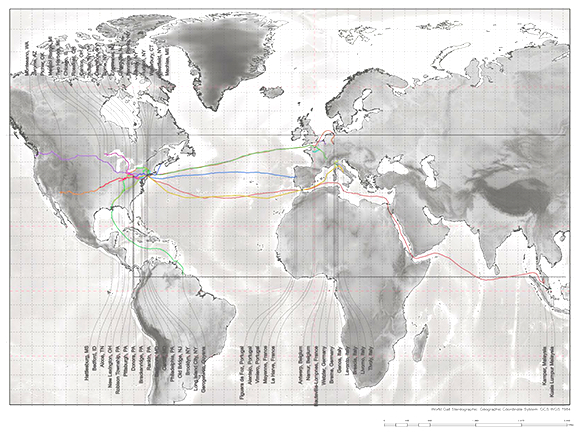
\includegraphics[width=1\linewidth]{figures/state.jpg}
    \caption{Provenance des matériaux et ressources nécessaires à la construction de l'Empire State Building en 1930. Carte réalisée en 2017 par Kiel Moe.}
    \label{fig:state}
\end{figure}
% Diaporama : conclusion de la séance 4 sans contenu, à compléter.


\backmatter
\printbibliography[heading=bibintoc]   % bibintoc = l'ajoute à la table des matières
\end{document}
